\documentclass[../main.tex]{subfiles}

\begin{document}
	\section{Sprints}
	\label{section:Sprint 0}
%Sprint 0
	\subsection{Sprint 0}
	
	\par Im ersten Sprint sind \gls{userstories} ausgewählt, die sich vor allem mit dem Aufsetzen der Infrastruktur und das beschaffen benötigter Daten für das Projekt befassen. Neben den üblichen Anforderungen (\gls{cicd}, \gls{versionierung} usw.) hat es auch noch eine User-Story für das Auseinandersetzen mit \gls{unity}. Da im Team der Wissensstand rund um Unity eher beschränkt ist, soll so die Wissensaneignung mit einkalkuliert werden. Wegen der eher kurzen Projektdauer, wurde die Sprint-Dauer auf 2 Wochen festgelegt.
	
	\begin{itemize}
		\item Initiale Produktdokumentation erstellen
		\item Infrastruktur aufsetzen
		\item \gls{testingpipeline} aufsetzen
		\item Sich mit Unity auseinandersetzen
	\end{itemize} 

	\par Das Team hat diese User-Stories in einzelne Tasks aufgeteilt. Ebenso haben alle Tasks Story-Points erhalten. Bei den \gls{storypoints} wird die \gls{fibonacciskala} verwendet, und die Punkte entsprechend dem minimalen Zeitaufwand
	
	\begin{center}
		 \begin{tabular}{c | c} 
			\hline
			Story-Points & Stundenwert \\ [0.5ex] 
			1 & 1 - 2 \\ [1ex] 
			2 & 2 - 3 \\ [1ex]
			3 & 3 - 5 \\ [1ex]
			5 & 5 - 8 \\ [1ex]
			8 & 8 - 16\\ [1ex] 
			\hline
		\end{tabular}
	\end{center}

	\par Die User-Stories sind wie folgt in Tasks aufgeteilt und mit Story-Points bewertet:
	
	\begin{itemize}
		\item Initiale Produktdokumentation erstellen
		\begin{itemize}
			\item Initiales Dokument kreieren [1]
			\item Rollen definieren [2]
			\item Technologien evaluieren und definieren [2]
			\item Initiale Architektur definieren [1]
			\item Hauptrisiken definieren und Vorgehen beschreiben [3]
			\item Kritikpunkte definieren, die das Produkt als erfolgreich bewerten [3]
			\item Hauptfeatures definieren [2]
			\item Detaillierten Beschrieb der Idee schreiben [1]
			\item Alles im PSIT4 Wiki Verlinken [1]
		\end{itemize} 
		\item Infrastruktur aufsetzen
		\begin{itemize}
			\item IDE bestimmen [1]
			\item Repositories auf GitHub erstellen [1]
			\item SonarQube mit GitHub verbinden [5]
			\item Automatisches bauen des Spiels auf GitHub implementieren [5]
			\item Hauptrisiken definieren und Vorgehen beschreiben [3]
			\item Kritikpunkte definieren, die das Produkt als erfolgreich bewerten [3]
			\item Hauptfeatures definieren [2]
			\item Detaillierten Beschrieb der Idee schreiben [1]
			\item Alles im PSIT4 Wiki Verlinken [1]
		\end{itemize} 
		\item Testing-Pipeline aufsetzen
		\begin{itemize}
			\item Automatisches testen auf GitHub implementieren [5]
		\end{itemize}
		\item Sich mit Unity auseinandersetzen
		\begin{itemize}
			\item Unity Prefabs [2]
			\item Unity Input System [2]
			\item Unity Camera System [2]
			\item Unity Testing [2]
		\end{itemize}
	\end{itemize} 

	\par Ebenfalls sind die Tasks auf die einzelnen Teammitgliedern aufgeteilt worden, sodass jeder in etwas gleich Ausgelastet ist. Trotzdem ist die Vereinbarung so, dass bei Bedarf natürlich mehrere Mitglieder am gleichen Task arbeiten können.


%Sprint 0 Review
	\subsubsection{Review}
	\label{section:Review}
	\par Der erste Sprint wurde mit einem Sprint-Review abgeschlossen. Dort wurde noch einmal der ganze Sprint überflogen sowie die einzelnen Tasks besprochen. Während des Sprints wurden durch die geringe Auslastung noch zwei Tasks, in Absprache mit PO und SM, hinzugefügt:
	
	\begin{itemize}
		\item Automatisches generieren der Dokumentation [2]
		\item Automatisches inkrementieren der Version [2]
	\end{itemize}

	Auch diese wurden Zeitgemäss ausgeführt. Dies ist ersichtlich im Burndown-Chart vom Sprint 0:
	
	\begin{figure}[H]
		\centering
		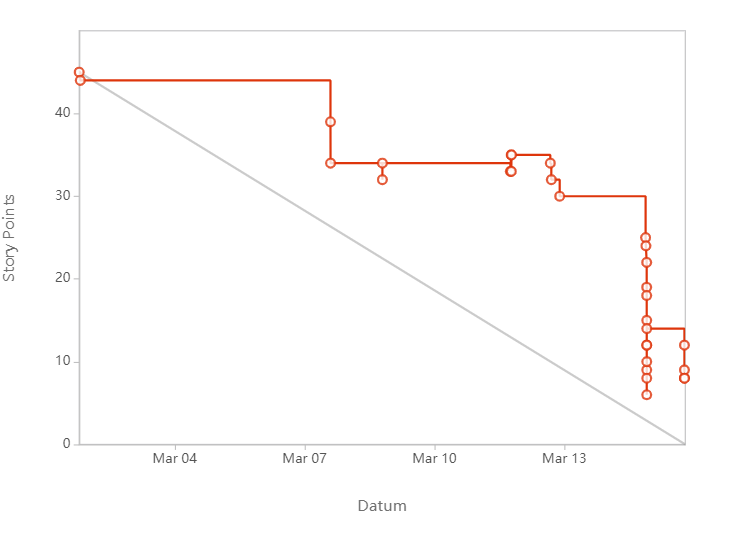
\includegraphics[width=0.5\textwidth]{Sprint_0_Burndown_Chart}
		\caption{Sprint 0 Burndown-Chart}
	\end{figure}

	\par Es gibt lediglich einen Task der nicht erfolgreich ausgeführt wurde, und zwar \textbf{SonarQube mit GitHub verbinden}. Hier waren über mehr als (kollektiv) 16 Stunden zwei Mitglieder am arbeiten, konnten aber keine nutzbare Integration erreichen. Nach Absprache mit dem PO wurde dies auch gestrichen. Für den nächsten Sprint wurde jedoch ein Task erstellt, um kurz nach Ausweichmöglichkeiten zu recherchieren.
	
	\par Gleichzeitig wurde im Sprint-Review durch das Team entschieden, das die User-Story \textbf{Sich mit Unity auseinandersetzen} bei jedem Sprint vorhanden sein wird. Dies soll den Overhead im Team darstellen, welches bei den einzelnen Tasks vorkommen kann.

\end{document}